%%%%%%%%%%%%%%%%%%%%%%%%%%%%%%%%%%%%%%%%%%%%%%%%%%%%%%%%%%%%%%%%%%%%%%%%%%%%%%%%%%%%
%Do not alter this block of commands.  If you're proficient at LaTeX, you may include additional packages, create macros, etc. immediately below this block of commands, but make sure to NOT alter the header, margin, and comment settings here. 
\documentclass[12pt]{article}
\usepackage{amsmath,amsthm,amssymb,amsfonts, enumitem, fancyhdr, color, comment, graphicx, environ, algorithm, algpseudocode}
%\usepackage{algorithmic}




%\pagestyle{fancy}
%\setlength{\headheight}{65pt}
\newenvironment{problem}[2][Problem]{\begin{trivlist}
\item[\hskip \labelsep {\bfseries #1}\hskip \labelsep {\bfseries #2.}]}{\end{trivlist}}
\newenvironment{sol}
    {\emph{Solution:}
    }
    {
    \qed
    }
\specialcomment{com}{ \color{blue} \textbf{Comment:} }{\color{black}} %for instructor comments while grading
\NewEnviron{probscore}{\marginpar{ \color{blue} \tiny Problem Score: \BODY \color{black} }}
%%%%%%%%%%%%%%%%%%%%%%%%%%%%%%%%%%%%%%%%%%%%%%%%%%%%%%%%%%%%%%%%%%%%%%%%%%%%%%%%%



%%%%%%%%%%%%%%%%%%%%%%%%%%%%%%%%%%%%%%
%Do not alter this block.
\begin{document}
%%%%%%%%%%%%%%%%%%%%%%%%%%%%%%%%%%%%%%

\title{Homework \#4 \\ CPSC 250 \\ Due: Friday, October 4th \\ Tanner Hammond}%replace X with the appropriate number
\date{}

\maketitle

%%%%%%%%%%%%%%%%%%%%%%%%%%%%%%%%DELETE%%%%%%%%%%%%%%%%%%%%%%%%%%%


%%%%%%%%%%%%%%%%%%%%%%%%%%%%%%%%%%%%%%DELETE%%%%%%%%%%%%%%%%%%%%%%%%%%%%%%%%%%%%%%%%%%%%%

\begin{enumerate}
\item (20) Give inductive proofs for the following statements:
\begin{enumerate}
\item $\Sigma_{i=1}^{n}(2i-1) = n^2$ \newline
\textbf{Base case}:When n = 1, the left side of it is 1 and the right side is 1. Both sides are equal and is true for n = 1. \newline
\textbf{Inductive step}:$\Sigma_{i = 1}^{n+1}(2i-1) = \Sigma_{i=1}^{n}(2i-1)+(2(n+1)-1)$\\
$=n^2 + 2(k+1)-1$\\
$=n^2 +2n + 1 = (n+1)^2$\newline
\textbf{Conclusion}:Thus it holds for n = n+1 and the proof of the induction step is complete. It is true for all n >= 2
\vspace{30px}
\item $\Sigma_{i=1}^{n}i^3 = (\frac{n(n+1)}{2})^2$\newline
\textbf{Base case}: When n=1, \newline
\textbf{Inductive step}:\newline
\textbf{Conclusion}:
\vspace{30px}
\end{enumerate}

\item (10) Arrange the following functions in ascending order of growth rates.
\begin{enumerate}
\item
$n, \sqrt{n}, n^{1.5}, n^2, n\lg n$
\begin{enumerate}
\item $\sqrt{n}$
\item $n$
\item $nlgn$
\item $n^1.5$
\item $n^2$
\end{enumerate}

\item
$n\lg\lg n, n\lg^2 n, 2/n, 2^n, 2^{n/2}$
\begin{enumerate}
\item $2/n$
\item $n\lg\lg n$
\item $n\lg^2 n$
\item $2^{n/2}$
\item $2^n$
\end{enumerate}

\item
$ 37, n^2\lg n, n^3, n \lg n^2, n^{2.01}$
\begin{enumerate}
\item $n\lg n^2$
\item $n^2\lg n$
\item $n^2$
\item $n^{2.01)$
\item $n^3$
\end{enumerate}

\end{enumerate}

\item (20) Prove that the following recursive algorithm works.
Assume that FIND-MAX-CROSSING-SUBARRAY($A, low, mid, high$) works. It returns a triple 
containing the indices demarcating a maximum subarray that crosses the midpoint, along with the 
sum of the values in a maximum subarray. You can read more of this problem on page 70 of the 
textbook.\newline
\textbf{Non-recursive case}: The only case where there is no recursive call is if low and high are equal to each other.
\vspace{30px}
\newline

\textbf{Recursive case}:If low and high aren't equal to each other, a mid point is created and the recursive calls start to find the maximum subarrays.\vspace{30px}
\newline

\textbf{Conclusion}:The recursive algorithm is true and does work.\vspace{30px}


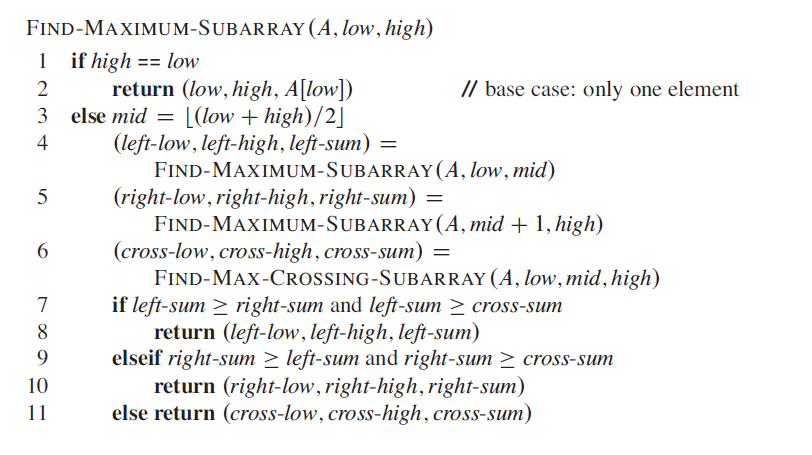
\includegraphics[width=1.0\textwidth]{maxsubarray.png}


\item(15) Design a quadratic time brute-force algorithm and linear time algorithm that takes an 
array $A$ of \textbf{positive} numbers that has \textbf{size at least 2}, and returns the 
maximum value of $A[j]- A[i]$, with $j > i$. Assume the array $A$ has an attribute $A.lenght$ 
that represents the size of the array. The array is indexed from 1 to $A.length$.
For example on of the array $A = [8,1,2,3]$ your algorithm should return 2. Since $A[4]- A[1]$
gives the largest difference and $4 > 1$. Note that the answer isn't $8-1 = 7$ since index 1 
isn't greater than index 2.

\begin{itemize}

\item \begin{algorithm}[H]
\begin{algorithmic}
\Procedure{Brute-Force-Pair-Difference}{$A$}
\State Brute Force!!!!!!!
\EndProcedure
\end{algorithmic}
\end{algorithm}

\item \begin{algorithm}[H]
\begin{algorithmic}
\Procedure{Efficient-Pair-Difference}{$A$}
\State Smart Force!!!!!!!
\EndProcedure
\end{algorithmic}
\end{algorithm}

\end{itemize}

\item (10) Consider the following code segments. Use it to answer the following questions.

\begin{algorithm}[H]
\begin{algorithmic}
\State \textbf{Code I}
\State
\State $i = 1$
\While{$i < n$}
 \State $i = 2 \times i$
\EndWhile
\end{algorithmic}
\end{algorithm}

\begin{algorithm}[H]
\begin{algorithmic}
\State \textbf{Code II}
\State
\While{$n > 0$}
 \State $n = \lfloor n/2 \rfloor$
\EndWhile
\end{algorithmic}
\end{algorithm}

\begin{enumerate}
\item If $n = 2^m$ for some nonnegative integer $m$, how many times does the while-loop
of \textbf{Code I} iterate?
\newline
Answer: $2^n$
\item If $n = 2^m + 1$ for some nonnegative integer $m$, how many times does the while-loop 
of \textbf{Code I} iterate?
\newline
Answer: $2^n + 1$
\item If $n = 2^m + r$ for some nonnegative integer $m$ and $0 < r < 2^m$, how many times does 
the while-loop of \textbf{Code I} iterate?
\newline
Answer: $2^n + r$
\item For any positive integer, how many times the while-loop of \textbf{Code I} iterate?
\newline Answer: $n$

\item Using asymptotic notation ($\Theta, O, o, \Omega, \omega,$) and input size $n$, what is the time complexity of \textbf{Code I} and \textbf{Code II}?\newline
Answer: $O(n/2)$
\end{enumerate}

\end{enumerate}

%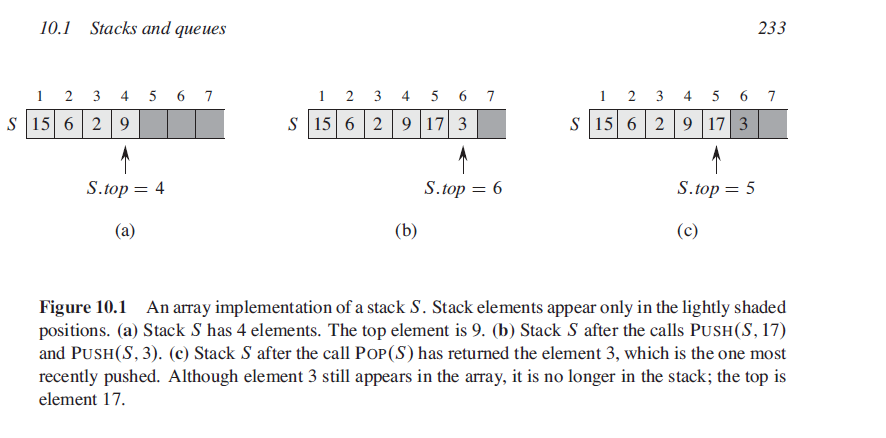
\includegraphics[width=1.0\textwidth]{fig_10_1}
%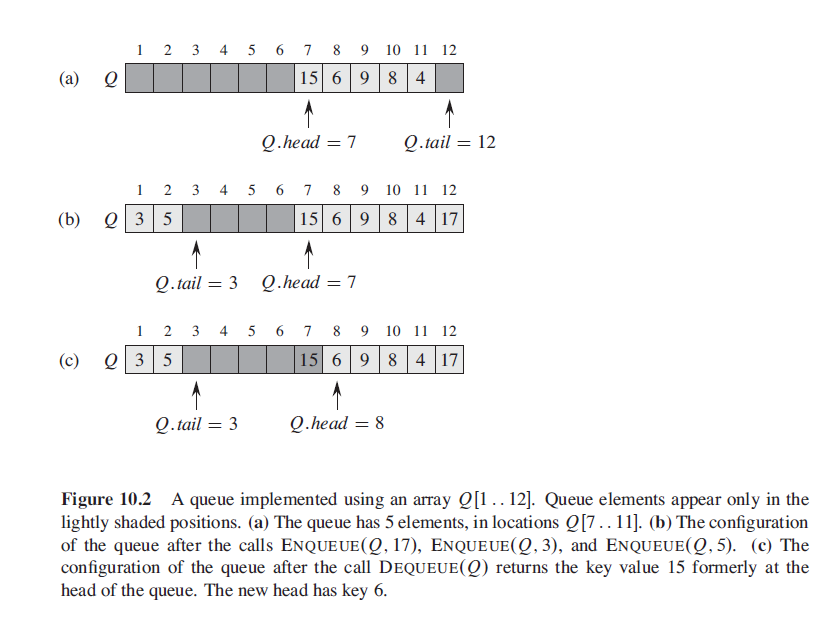
\includegraphics[width=1.0\textwidth]{fig_10_2}
%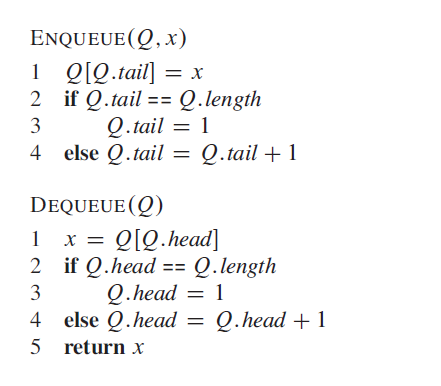
\includegraphics[width=1.0\textwidth]{EnqueueDequeue}


%Copy the following block of text for each problem in the assignment.
%\begin{problem}{1}
%\end{problem}
%%%%%%%%%%%%%%%%%%%%%%%%%%%%%%%%%%%%%%%%
%Do not alter anything below this line.
\end{document}